\chapter{Planejamento da Expansão de Sistemas de Distribuição}
\label{chp:pesd}

Neste capítulo, são apresentados os principais conceitos e aspectos do \ac{PESD}. Inicialmente é descrito como a regulação brasileira define as etapas de \ac{PESD} segundo os \ac{PRODIST} -- Módulo 2 da \citeonline{prodist2}, no âmbito desta regulação, a área de pesquisa desenvolvida neste trabalho é situada. Em seguida, esta área de pesquisa é descrita, em linhas gerais, como um problema de otimização, definindo algumas abstrações das restrições e de tipos de função objetivo para um melhor entendimento do problema. Após esta introdução ao problema de \ac{PESD}, são discutidos os modelos matemáticos encontrados na literatura e a justificativa da utilização do modelo base deste trabalho. Por fim, é apresentado detalhadamente o modelo utilizado, descrevendo os lados positivos e negativos do mesmo.

Conforme citado no capítulo anterior, este trabalho utiliza um modelo linear-inteiro misto do problema de \ac{PESD}. Este modelo foi inicialmente proposto por \citeonline{Haffner2008} e vem sendo desenvolvido (e expandido), entre outros, pelos pesquisadores da Universidad de Castilla-La Mancha como pode ser visto nos trabalhos de \citeonline{Lotero2011}, \citeonline{MunozDelgado2015}, e \citeonline{Asensio2018}. No geral, o modelo representa um planejamento multiestágio, visando minimizar o valor presente líquido dos investimentos e custos com a expansão do sistema de distribuição. O modelo é baseado em uma linearização das equações de fluxo de potência e de perdas, considerando injeções de corrente, e a utilização de injeções de correntes fictícias para garantir a radialidade do sistema de distribuição enquanto a empresa distribuidora também planeja a alocação de geração distribuída.

Ao final deste capítulo, espera-se que os principais aspectos do PESD estejam claros para o leitor, bem como as principais características do problema de PESD em sua formulação matemática e os detalhes do modelo utilizado neste trabalho.



\section{Etapas do planejamento da expansão de sistemas de distribuição}


A distribuição de energia elétrica é a penúltima etapa dentre as etapas de geração, transmissão, distribuição e consumo de energia elétrica. O sistema de distribuição de energia elétrica é o responsável por ajustar o nível de tensão da etapa de transmissão para o nível de tensão da etapa do consumo, entregando a energia demandada com qualidade seguindo as normas locais. 

No sistema de distribuição há várias características que os diferenciam dos sistemas de transmissão, que acarretam em outros desafios para o planejamento da expansão e operação. Dentre essas características, pode-se elencar as seguintes:

\begin{itemize}
    \item fluxo de potência direcional: Mesmo com o aumento da presença de geradores distribuídos ao longo do sistema de distribuição, o fluxo de potência na direção da subestação para o consumidor ainda é majoritário em sistemas de distribuição. Porém, cada vez mais este cenário tem mudado, e não é incomum empresas de distribuição relatarem problemas de fluxo de potência reverso causado em situações de baixo carregamento;
    
    \item topologia radial: Sistemas de distribuição radiais são a maioria. Esta topologia facilita a manutenção destes sistemas, principalmente devido à característica do fluxo de potência direcional;
    
    \item perfil de tensão: Devido à topologia e fluxo de potência, o nível de tensão em sistemas de distribuição tem o comportamento de ir reduzindo ao longo do alimentador. Caracterizando uma constante preocupação da empresa distribuidora com os níveis de tensão;
    
    \item comprimento do sistema e linhas: Em relação aos sistemas de transmissão, os sistemas de distribuição tem um menor comprimento e são caracterizados por linhas com menor seção transversal, o que aumenta a resistência elétrica e as perdas técnicas. 
\end{itemize}

No Brasil, as empresas distribuidoras (responsáveis pelo sistema de distribuição) devem seguir as normas descritas nos 11 módulos dos \ac{PRODIST} da \citeonline{ANEELPRODIST}, estes módulos descrevem os procedimentos desde o PESD até o faturamento da energia elétrica.

O \ac{PESD} é o planejamento das ações a serem realizadas pela empresa distribuidora para atender o crescimento da demanda de uma determinada região com qualidade. Estas ações são guiadas por um plano de execução que seleciona as atividades e a ordem em que serão executadas durante e após a execução do plano. Desta forma, o \ac{PESD} permite que a empresa distribuidora opere de forma segura o sistema de distribuição resultante.

Especificamente, o Módulo 2 da \citeonline{prodist2} descreve os procedimentos para \ac{PESD}.  Nesta norma, o \ac{PESD} é dividido em quatro etapas em que as três primeiras etapas devem ser compiladas em um plano (última etapa) e este plano é reportado à \ac{ANEEL}. Cada etapa é descrita a seguir:

\begin{enumerate}
    \item Previsão de demanda, na qual a empresa distribuidora desenvolve estudos de previsão de carga de médio e longo prazo, considerando a periodicidade e, no mínimo, o histórico consolidado de cargas dos últimos anos, de forma que forneça as informações necessárias para o planejamento de linhas e subestações. 
    
    \item Caracterização da carga e do sistema elétrico, na qual, utilizando campanhas de medição, as unidades consumidoras são estratificadas para a realização da caracterização da curva de carga e dos alimentadores da rede e transformadores do sistema de distribuição. 

    \item Critérios e estudos de planejamento, no qual são realizados estudos técnicos e econômicos necessários para a definição dos esforços e investimentos a fim de atender aos consumidores. Nesta etapa, é realizada a escolha de todas as linhas, subestações e outros equipamentos que serão instalados no sistema de distribuição.
    
    \item Plano de desenvolvimento da distribuição, descreve os estudos realizados e os planos de obras que serão implementados na expansão. Este plano é entregue anualmente à ANEEL, apresentando o conjunto de obras do ano e as obras dos anos seguintes.

\end{enumerate}

Logo, podemos situar a área de pesquisa do problema de \ac{PESD} na Etapa 3. Esta etapa assume que as cargas já passaram por um processo de previsão e caracterização, tendo a empresa distribuidora o objetivo de selecionar quais possibilidades de alimentadores serão utilizados, as linhas, se há a necessidade de expansão ou até construção de novas subestações e a instalação de outros equipamentos, como de regulação de tensão ou proteção. O plano de desenvolvimento da distribuição foge do escopo desta área de pesquisa, visto que a decisão final das obras e o desenvolvimento do documento devem ser realizados à luz da estratégia da empresa, dos interesses dos controladores e outros \textit{stakeholders}.



\section{Introdução ao problema matemático}


Em linhas gerais, o problema clássico de \ac{PESD} consiste na determinação da localização e estágio de instalação de novos equipamentos, como linhas, transformadores, etc. Este problema também inclui a possibilidade da criação de novas ou expansão de subestações existentes. No plano resultante do problema, deve-se considerar os limites operacionais de cada equipamento, limites de tensão e capacidade de acomodar as novas cargas previstas. Geralmente, considera-se minimizar os custos com investimentos, com restrições relacionadas aos limites operacionais e ao atendimento das cargas com qualidade de energia.

Este problema de atender todas as cargas com qualidade e respeitando o limite operacional enquanto busca-se um plano de expansão com o menor custo possível, pode ser descrito como um problema de otimização matemática (ou programação matemática), visto que as equações que regem o comportamento em regime permanente de sistemas elétricos de potência são bem conhecidas. Os detalhes destes equacionamentos estão bem descritos no livro de \citeonline{monticelli1983fluxo} e mais especificamente para sistemas de distribuição no livro de \citeonline{kersting2017distribution}.

Não é o objetivo deste trabalho explicar detalhadamente a estrutura e conceitos relacionados à otimização matemática. Porém, é importante definir alguns conceitos básicos para um melhor entendimento do problema de \ac{PESD}. Caso haja interesse do leitor, aconselha-se o livro de \citeonline{2006pesquisa}. Desta forma, define-se os seguintes conceitos:

\begin{itemize}
    \item Variáveis: dados que devem ser definidos a fim de solucionar o problema. Ex: entre três investimentos, em quais (variáveis) e quanto (variáveis) se deve investir (problema)?
    
    \item Função objetivo: função que descreve, por meio das variáveis  e parâmetros do problema, a métrica de avaliação da decisão. Ex: custos relacionados aos investimentos.
    
    \item Restrições: conjunto de equações que delimitam o problema, ou impõem limites às decisões. Ex: os investimentos não podem superar um valor de risco máximo.
    
    \item Modelo (ou modelagem): conjunto de equações, composto por função objetivo, restrições, variáveis e parâmetros do problema, que descrevem o comportamento relevante de um sistema ou problema real.
    
    \item Programação inteira-mista: são problemas de otimização em que as variáveis são representadas por números do conjunto dos inteiros ou reais.
\end{itemize}


Dada estas definições, o problema de \ac{PESD} pode ser representado em modelos de programação inteira-mista, no qual as variáveis de decisão de investimentos (novas linhas, novos transformadores, expansão de subestações, etc.) podem ser representadas como variáveis binárias (1 se a decisão for tomada e 0 se não) e as variáveis que descrevem o comportamento do sistema de distribuição (tensão, corrente, potência, perdas) podem ser representadas como variáveis reais e relacionadas entre si por meio de restrições (balanço de potência, leis de Kirchhoff, etc.). 

Restrições lógicas que descrevem o comportamento das decisões de investimento também devem ser incluídas no problema. Estas restrições têm por objetivo evitar, por exemplo, que duas linhas sejam instaladas entre dois barramentos do sistema, ou que um novo transformador de subestação seja instalado sem que a subestação seja construída. Em conjunto, restrições de investimentos também podem ser adicionadas para evitar custos elevados em um único estágio ou qualquer outra questão financeira do problema.

Especificamente para sistemas de distribuição, um conjunto de restrições a mais é adicionado ao modelo, referente à radialidade do sistema, característica majoritária conforme descrito anteriormente. A função objetivo do problema já é definida como os custos relacionados aos investimentos, e portanto pode ser facilmente obtida através de métricas de investimentos, como \ac{VPL} dos investimentos.

Uma observação relevante na métrica de investimento é que nem todos os trabalhos de \ac{PESD} utilizam apenas o \ac{VPL} dos investimentos como a métrica para a tomada de decisão de um investimento, dentre estes trabalhos destacam-se os trabalhos de \citeonline{7462292} que inclui uma métrica monetária de bem estar social dada a mudança do sistema e \citeonline{HOMEORTIZ201986} que incluí uma métrica monetária de emissão de dióxido de carbono.

Por fim, restrições de domínio são adicionadas para delimitar o conjunto de números das variáveis (reais, inteiras, binárias ou subconjuntos).

Logo, podemos generalizar o problema clássico de \ac{PESD} conforme descrito em \eqref{eq:modelo}:
\begin{align}
        \label{eq:modelo}
        \text{min./max. }& \text{Métrica de investimento} \nonumber\\
        \text{s.a. }& \text{Comportamento do sistema}\nonumber\\
                    & \text{Limites operacionais} \nonumber\\
                    & \text{Radialidade}\\
                    & \text{Restrições lógicas} \nonumber \\
                    & \text{Restrições de investimentos}\nonumber\\
                    & \text{Restrições de domínio}\nonumber
\end{align}

A notação utilizada em \eqref{eq:modelo} pode ser lida como: minimize (ou maximize, dependendo do modelo) a métrica de investimento sujeito às restrições de comportamento do sistema, limites operacionais, radialidade, restrições lógicas, restrições de investimentos e restrições de domínio. Na próxima seção, serão discutidos os diferentes modelos encontrados na literatura e suas principais contribuições para o desenvolvimento do problema de \ac{PESD}.
\vfill

\section{Modelos matemáticos do problema na literatura acadêmica}

O problema de \ac{PESD} vem há muito tempo sendo discutido na literatura. No trabalho de \citeonline{TEMRAZ199361}, é realizado um levantamento dos 24 principais trabalhos realizados durante meados da década de 1960 até início da década de 1990. Neste trabalho, cada artigo foi classificado em dois diferentes eixos: estático -- dinâmico e subsistemas -- sistema inteiro, no qual o modelo ou método de solução considera estático quando apenas um estágio do planejamento é realizado e dinâmico quando mais de um estágio é considerado. O segundo eixo se refere a métodos ou modelos que consideram todo o sistema de distribuição a ser planejado ou dividem o sistema de distribuição em subsistemas e os planejam.


Dentre os trabalhos, ressalta-se o algoritmo proposto por \citeonline{4766010}, que utiliza o menor caminho para determinar a topologia do sistema de distribuição e decide sobre transformadores através da quantidade de carga demandada. Já no modelo proposto por \citeonline{Adams1973} é descrito a primeira utilização de métodos de programação matemática para a resolução do problema de \ac{PESD} através de programação dinâmica considerando multiestágios.  Considerando programação linear, destaca-se o modelo proposto por \citeonline{4113575}, que utiliza um modelo linear de logística e o ressignifica para o problema de \ac{PESD}. Em programação inteira, o trabalho de \citeonline{4075490} utiliza um método iterativo binário para selecionar as linhas e as subestações através de otimização. Por fim, o trabalho de \citeonline{Gonen1981} descreve um dos primeiros registros de um modelo matemático de programação inteira-mista que planeja tanto a subestação, quanto as linhas do sistema de distribuição.


Observa-se nos trabalhos desenvolvidos até o início da década de 1990 um desenvolvimento de métodos de solução que utilizam tanto modelos matemáticos quanto algoritmos heurísticos que utilizavam alguma outra informação do problema. Outro aspecto relevante destes trabalhos foi o desenvolvimento de métodos quando não havia tantos recursos computacionais quanto há atualmente. Vários destes artigos relatam a dificuldade e as restrições dos recursos computacionais da época, o que impactava diretamente no tamanho dos problemas testes e na quantidade de aproximações realizadas.


Entre meados da década de 1990 até meados da década de 2000 surge a utilização de métodos inteligentes e meta-heurísticos para sua solução. Estes métodos começaram a ser utilizados devido às aproximações que estavam sendo realizadas para considerar as não-linearidades do problema de \ac{PESD}, principalmente relacionadas às equações que regem o comportamento do sistema de distribuição.

Algoritmo Genético foi empregado por \citeonline{331452} para a determinação das linhas e das subestações, no qual as restrições do comportamento do sistema eram satisfeitas através da resolução do problema de fluxo de potência. Já \citeonline{667402} expandiu esse conceito para sistemas de distribuição maiores demonstrando a eficiência do método. Já em \citeonline{1295010}, foi utilizado o algoritmo de colônia de formigas em sistemas de distribuição com um grande número de barramentos e decisões, os resultados tiveram a eficiência próxima aos de \citeonline{667402}. A utilização de métodos meta-heurísticos se consolidou na área e \citeonline{8995556} demonstra que atualmente encontra-se diversos estudos que continuam demonstrando a flexibilidade e eficácia do uso desses métodos no problema de \ac{PESD}.


A partir de meados da década de 2000 até meados da década de 2010 a presença de geradores distribuídos começou a ser amplamente considerada nos modelos de \ac{PESD}. Em \citeonline{Haffner2008} foi proposto um modelo para o problema de \ac{PESD} que pela primeira vez unia em um só modelo linear inteiro-misto: planejamento multiestágio, limites operacionais de equipamentos, adição e substituição de linhas, expansão e novas construções de subestações, limites de tensão e incluía geração distribuída, porém sem planejar sua alocação. Este modelo será melhor discutido na próxima seção.

A proposta de \citeonline{Haffner2008}, foi a base para o método de solução proposto por \citeonline{Lotero2011} que incluía confiabilidade e uma linearização por partes para considerar perdas. A partir deste trabalho, o modelo proposto por \citeonline{Haffner2008} seria expandido para diversas outras aplicações dando início a sequência de trabalhos realizados pelos pesquisadores da Universidad de Castilla-La Mancha.


Entretanto, o trabalho de \citeonline{5982115} consolidou e aprofundou a discussão em relação às restrições de radialidade, não apenas nos modelos de \ac{PESD}, mas em diversos problemas de otimização em sistemas de distribuição. Dentre os problemas em relação ao \ac{PESD} se tornou evidente a questão de ilhamentos alimentados apenas com geradores distribuídos, visto que as restrições de radialidade tradicionalmente utilizadas não evitavam essas situações. Este problema seria superado a partir do trabalho de \citeonline{MunozDelgado2015}, que utilizando injeções de corrente fictícias, desenvolveu um modelo baseado na proposta de \citeonline{Haffner2008} que incluía o planejamento de geradores distribuídos junto com o \ac{PESD}.

Durante o mesmo período, os métodos meta-heurísticos continuaram sendo utilizados para solucionar as equações não lineares do problema de \ac{PESD}. Destacam-se os trabalhos de \citeonline{6203389} que utilizam algoritmo genético e fluxo de potência ótimo para encontrar uma topologia do sistema de distribuição; \citeonline{6450147}, que abordam um modelo não linear inteiro misto e uma modificação do algoritmo de otimização por enxame de partículas; e por fim, \citeonline{Benvindo2014} que utiliza busca tabu para a resolução do problema de \ac{PESD}.


Desde meados da década de 2010 até atualmente, muitos avanços nos modelos do problema do \ac{PESD} foram realizados. Destaca-se os modelos quadráticos e cônicos, que apesar de serem não lineares, apresentam boa convergência e possuem métodos de solução conhecidos. O trabalho de \citeonline{6387348} propõe a utilização de um modelo quadrático com uma formulação poliedral que permitia, através de eliminação de restrições, ser solucionada por \textit{solvers} comerciais. Em contraste a esta abordagem, o trabalho de \citeonline{FRANCO2014265} propõe a utilização das variáveis originais de fluxo de potência em um modelo quadrático em conjunto com a alocação de banco de capacitores. Já o trabalho \citeonline{7422914} propõe a utilização de uma modelagem cônica de segunda ordem em conjunto com relaxação de restrições, integrando a alocação de sistemas de armazenamento de energia. Esta abordagem foi complementada por \citeonline{XIE2020105451} que integrou o gerenciamento de sistemas de distribuição ativos.


Durante a mesma época, diversos trabalhos iniciaram a integração de novas cargas e novos ativos no problema de \ac{PESD} a partir do modelo proposto por \citeonline{Haffner2008}. No trabalho de \citeonline{7353222} a integração entre \ac{PESD}, geradores distribuídos e confiabilidade foi realizado através de um \textit{framework} inspirado no trabalho de \citeonline{Lotero2011}. Já em \citeonline{7462292} um modelo estocástico baseado em maximizar o benefício social foi proposto para a integração do planejamento de geradores distribuídos, \ac{PESD}, armazenamento de energia com resposta a demanda dentro de um mesmo modelo. 

Recentemente, no trabalho de \citeonline{8636266}, inspirado na proposta de \citeonline{PORKAR2010828} em que geradores distribuídos são planejados em conjunto com o \ac{PESD} na perspectiva de um mercado não regulado, é proposta uma abordagem de três níveis para o problema de \ac{PESD}, na presença de geradores distribuídos que operam de forma independente. Nesta abordagem, há três atores: a empresa distribuidora, os donos dos geradores distribuídos e os operadores independentes. A empresa distribuidora é responsável pela expansão do sistema de distribuição, na qual permite que os donos dos geradores distribuídos escolham o investimento em geradores distribuídos e se inicie a operação de despacho dos geradores distribuídos pelos operadores independentes.

Observa-se que o modelo proposto inicialmente por \citeonline{Haffner2008} tem sido aprimorado ano a ano e vêm abordando diversos novos aspectos em seu desenvolvimento. Sua adesão deve-se à fácil implementação e solução em diversos tipos de \textit{solvers} comerciais, por utilizar um modelo linear inteiro-misto suficientemente próximo às práticas utilizadas por engenheiros de planejamento. Estes dois motivos foram os impulsionadores para a sua escolha de implementação neste trabalho.



% \subsection{Os modelos, as incertezas e a operação de sistemas de distribuição}

% \todo

\section{O modelo matemático base do trabalho}

Esta seção descreve o modelo utilizado para o \ac{PESD}. Nesta pesquisa, o planejamento é modelado como um problema de otimização linear inteiro misto, seguindo a mesma linha de desenvolvimento inicialmente proposta na forma matricial por \citeonline{Haffner2008}, adaptada algebricamente e complementada por \citeonline{MunozDelgado2015}.

O modelo utilizado nesta pesquisa prevê a inclusão e substituição de novos ramos e condutores no sistema, construção ou expansão de subestações, instalação de novos transformadores e geradores distribuídos. Adicionalmente, inclui os gastos com a manutenção desses equipamentos, custos com manutenção e de geração de energia. Diferente do modelo proposto por \citeonline{MunozDelgado2015}, os custos com demanda não suprida não são incluídos no modelo, pois não é permitido demanda não suprida no modelo proposto\footnote{A decisão de não permitir demanda não suprida foi tomada devido a necessidade de encontrar várias soluções que atendam a todos os consumidores, a fim de analisar o \ac{HC}. Se o modelo permitisse demanda não suprida, a maioria das soluções encontradas poderiam ser baseadas em demanda não suprida, o que desviaria da finalidade de \ac{HC} em que a operação atende a todos os consumidores.}. 

Nesta modelagem, o sistema de distribuição é subdividido em ramos e nós. Os ramos são identificados pelos nós dos quais se liga ($s$ e $r$), tipo de ramo e condutores ($l$), alternativa ($k$) e estágio ($t$).

% A figura \ref{fig:ramos} apresenta exemplos de ramos e nós de acordo com cada tipo.

% \begin{figure}[ht]	
% % 	\centering
%     \caption{Representação do modelo de ramos entre dois nós ($y^l_{srkt}$) em um estágio $t$, para ramos: (a) que podem ser substituídos; (b) que podem ser incluídos; (c) fixos}
% 	\centering
%     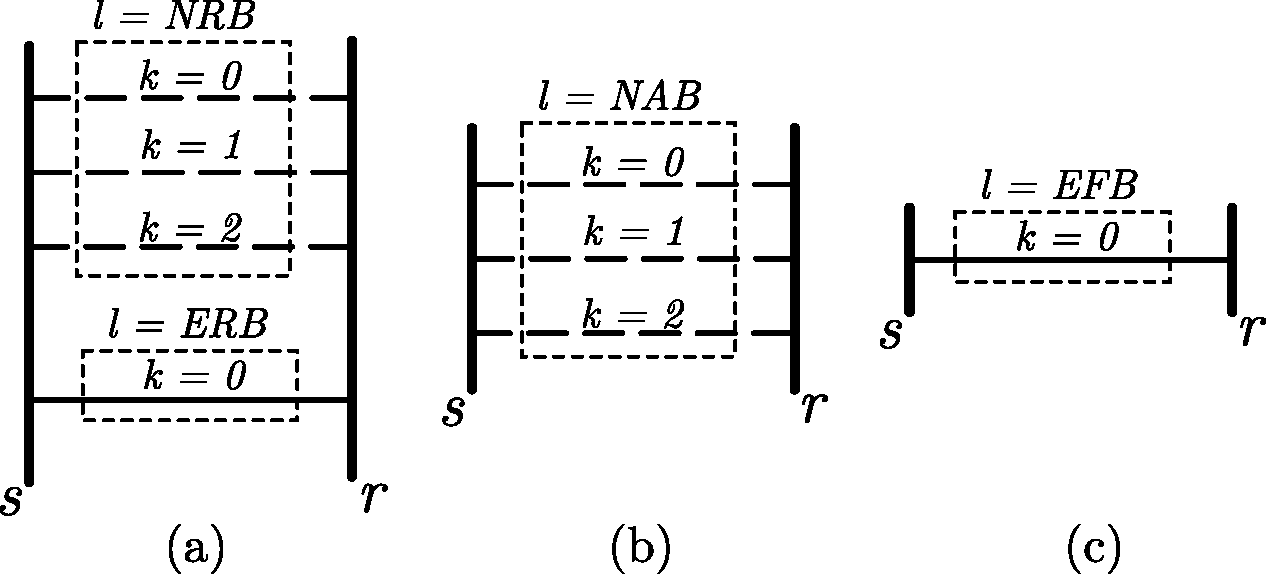
\includegraphics[width=0.8\textwidth]{cap2/ramos.pdf}
%     \\\vspace{1em}Fonte: Proprio Autor
%     \label{fig:ramos}
% \end{figure}

Note que entre dois nós, pode haver mais de um tipo de condutor. Este caso ocorre apenas para os ramos que podem ser substituíveis, visto que há o conjunto de condutores existentes ($ERF$) e novos ($NRF$). Nos outros tipos de ramos há apenas um tipo de condutor, seja novo para ser incluído ($NAF$) ou existente fixo ($EFF$). Os ramos para inclusão não estão fisicamente no sistema de distribuição antes da expansão e podem ser incluídos durante a expansão. Já os ramos existentes fixos estão previamente no sistema de distribuição e não podem sofrer alterações durante a execução do plano de expansão.

Do ponto de vista da modelagem matemática, não há diferença entre ramos e condutores, visto que todos os ramos/condutores são indexados nas mesmas variáveis. Nesta modelagem, todos os ramos/condutores estão conectados no sistema de distribuição e a variável  $y^l_{srkt}$ é responsável por "acionar" \; esses condutores. A solução do modelo retorna quais condutores serão "acionados"  \; (abstração de escolhidos) para a conexão de nós em cada estágio do plano de expansão.

De forma análoga, a abstração de acionamento é modelada também para a construção de subestações, instalação de novos transformadores e geradores distribuídos. Este tipo de modelagem permite a utilização de variáveis binárias em que 0 significa que o equipamento não será instalado e 1 significa que será instalado.

Este modelo também utiliza a linearização do comportamento do sistema de distribuição proposta por \citeonline{Haffner2008} que avalia o sistema de distribuição pela injeção de corrente de cargas, transformadores e geradores distribuídos. Esta linearização é uma versão adaptada do modelo de sistemas de transmissão e pressupõem que: todas as correntes possuem o mesmo fator de potência e a diferença de tensão entre os dois nós é igual a diferença do módulo de tensão entre eles. 
Nas subseções a seguir serão descritos os equacionamentos matemáticos do modelo, explicando a função objetivo, restrições e as alterações que foram implementadas durante o andamento desta pesquisa.

\subsection{Função objetivo}
\label{sec:fobj}

A função objetivo do modelo de \ac{PESD} utilizado é expressada nas equações \eqref{eq:fobj} e \eqref{eq:descriFobj}, nas quais representam o valor presente do custo total do plano de expansão. Essa função objetivo assume que os custos de investimentos são amortizados para cada estágio do planejamento e todos os equipamentos instalados são utilizados até o final de suas vidas úteis e substituídos por outro idêntico. Também considera-se que cada estágio tem duração de um ano ao assumir uma taxa de juros anual. Esse mesmo tipo de formulação é utilizada nos trabalhos de \citeonline{Lotero2011}, \citeonline{MunozDelgado2015}  e \citeonline{7462292}.
\begin{equation}
    \text{min     } c^{TPV}
    \label{eq:fobj}
\end{equation}
\begin{align}
     c^{TPV}  = & \sum_{t\in T} \left[ \frac{(i +i)^{-t}}{i} c^I_t + (i +i)^{-t} (c^M_t + c^E_t+ c^R_t)\right] 
       +\frac{(i +i)^{-n_T}}{i} (c^M_{n_T}  + c^E_{n_T} + c^R_{n_T})
     \label{eq:descriFobj}
\end{align}

Como pode ser visto, o modelo não utiliza energia não suprida em seu equacionamento. Esta escolha de modelagem força o modelo a sempre atender todas as cargas do plano e reduz o espaço de busca por uma solução. 
Cada custo considerado é expresso nas equações de \eqref{eq:invest} a \eqref{eq:perdas}, nas quais, cada item de investimento, manutenção, energia e perdas possui custos fixos associados a sua classe.

Cada custo de investimento possui fatores de conversão para o \ac{VPL}, conforme a indicado a seguir: $RR^l = (i(1+i)^{\eta^l})/((1+i)^{\eta^l} - 1), \forall l \in \{NFB, NAB\}$; $RR^{NT} = (i(1+i)^{\eta^{NT}})/((1+i)^{\eta^{NT}} - 1)$;
$RR^{DG}_p = (i(1+i)^{\eta^{DG}_p})/((1+i)^{\eta^{DG}_p} - 1)$; $RR^{SS} = (i(1+i)^{\eta^{SS}})/((1+i)^{\eta^{SS}} - 1)$. Estes fatores de conversão consideram que ao final da vida útil de cada equipamento, ele será substituído por outro idêntico até o fim do horizonte de planejamento.

Em \eqref{eq:invest} o custo com investimento para cada estágio é formulado. Os investimentos que podem ser realizados são: substituição ou adição de novas linhas, expansão de subestações existentes e adição de novas, instalação de novos transformadores nas subestações e instalação de geradores distribuídos.

% Diferente do modelo de \citeonline{MunozDelgado2015}, são considerados apenas geradores distribuídos despacháveis. Esta consideração é realizada devido a necessidade da empresa distribuidora poder controlar a potência injetada de cada gerador distribuído e assim ter uma segurança sobre a operação do sistema no contexto de \ac{HC}. Outro motivo é devido ao modelo original não lidar com o comportamento estocástico de geradores distribuídos de fontes renováveis e, na opinião do autor, isto acaba sendo uma aproximação que pode ocasionar outros problemas durante a operação do sistema de distribuição planejado. Por outro lado, formulações que consideram o comportamento estocástico de geradores distribuídos de fontes renováveis costumam aumentar consideravelmente a quantidade de variáveis de decisão e restrições, dificultando assim a resolução do problema de \ac{PESD}, como pode ser visto no trabalho de \citeonline{Asensio2018}.

\begin{align}
     c^I_t  = & \sum_{l\in \{NRB, NAB\}} RR^l  \sum_{k\in K^l} \sum_{(s,r)\in \Upsilon^l}C^{I,l}_k \ell_{sr}x^l_{srkt}
     + RR^{SS}  \sum_{s \in \Omega^{SS}} C^{I,SS}_k x^{SS}_{st} \nonumber\\
     &+ RR^{NT}  \sum_{k\in K^{NT}} \sum_{s \in \Omega^{SS}}  C^{I,NT}_k x^{NT}_{st}
     +\sum_{p\in P}  RR^{DG}_p \sum_{k\in K^{DG}_p} \sum_{s \in \Omega^{DG}_p} C^{I,DG}_{pk} pf\overline{G}^{DG}_{pk} x^{DG}_{pskt};\nonumber\\ &\forall t \in T
     \label{eq:invest}
\end{align}

Em \eqref{eq:manu} descreve-se os custos com a manutenção de cada elemento utilizado no sistema de distribuição. Da mesma forma que o equacionamento dos investimentos, cada elemento utilizado possui o custo fixo de manutenção. 

\begin{align}
     c^M_t  = & \sum_{l\in L}  \sum_{k\in K^l} \sum_{(s,r)\in \Upsilon^l} C^{M,l}_k (y^l_{srkt} + y^l_{rskt})
     + \sum_{tr \in TR} \sum_{k\in K^{tr}} \sum_{s \in \Omega^{SS}} C^{M,tr}_k y^{tr}_{skt}\nonumber\\
     &+ \sum_{p\in P} \sum_{k\in K^{DG}_p}\sum_{s \in \Omega^{DG}_p} C^{M,DG}_{pk} y^{DG}_{pskt}; \; \; \forall t \in T
     \label{eq:manu}
\end{align}

Em \eqref{eq:energia} apresenta-se o custo com produção de energia.\footnote{Durante as simulações realizadas para a implementação do modelo base do problema de \ac{PESD}, foi observado que a consideração do custo de produção de energia causa alguns problemas de convergência para a solução ótima do modelo ao se utilizar a estratégia de \textit{gap} relativo (ou tolerância absoluta relativa) no algoritmo de Branch \& Bound.
Ao se utilizar um gap de 0,1\% (a fim de se aproximar da solução ótima do problema) os custos com energia se mantém próximos à solução de 1\% reportada no artigo original, porém, os outros custos, opções de investimento e a topologia do sistema de distribuição são completamente diferentes e o tempo computacional aumenta exponencialmente com a redução do valor de gap. Isto ocorre devido aos custos de produção de energia serem mais de 85\% dos custos totais das soluções encontradas durante as simulações. Por outro lado, não considerar os custos de produção de energia torna indiferente uma das maiores vantagens de geradores distribuídos baseados em eólico e solar: não haver custos de geração, apenas manutenção. Desta forma, foi decidido manter este custo com produção de energia.}, seja da compra de energia provinda da transmissão, seja pela geração distribuída instalada

\begin{align}
    c^E_t  =
    \sum_{b \in B} \Delta_b pf\bigg[
    \sum_{tr \in TR} \sum_{k \in K^{tr}} \sum_{s \in \Omega^{SS}}
    C^{SS}_b g^{tr}_{sktbh} + 
    \sum_{p \in P}\sum_{k \in K^{DG}_p} \sum_{s \in \Omega^{DG}_p} C^{E, \;DG}_{pk}  g^{DG}_{psktbh}\bigg]; \nonumber\; \;\\ \forall t \in T, h=E 
    \label{eq:energia}
\end{align}
 

Em \eqref{eq:perdas} são equacionadas as perdas relacionadas aos transformadores e linhas utilizadas. Como pode-se observar há dois fatores quadráticos no problema e segundo \citeonline{Lotero2011} e \citeonline{MunozDelgado2015} a presença destes dois fatores pode causar dificuldades na busca por soluções do problema. 

\begin{align}
 c^R_t  =
\sum_{b \in B} C^{SS}_b \Delta_b pf \bigg[&\sum_{tr \in TR} \sum_{k \in K^{tr}} \sum_{s \in \Omega^{SS}} Z^{tr}_k (g^{tr}_{sktbh})^2  +\nonumber \\
&\sum_{l \in L} \sum_{k \in K^l} \sum_{(s, r) \in \Upsilon^l} Z^l \ell_{sr} (f^l_{srktbh} + f^l_{rsktbh})^2
\bigg]; \; \; \forall t \in T, h=E 
\label{eq:perdas}
\end{align}

Desta forma, é demonstrada  a seguir a estratégia utilizada para a linearização dos termos quadráticos. 

\subsubsection*{Linearização das perdas}

Os termos quadráticos são linearizados conforme descrito e utilizado por \citeonline{Gonen1981, Lotero2011, MunozDelgado2015}. Esta estratégia utiliza a linearização por partes e mais detalhes podem ser vistos em \citeonline{Gonen1981}. Desta forma a equação \eqref{eq:perdas} é substituída pelas equações de \eqref{eq:perdas_lin} a \eqref{eq:perdas_lin2}. No modelo proposto, o parâmetros da linearização são definidos como: $M^{l}_{k\nu} = (2\nu - 1)Z^l_k \overline{F}^l_k/n_\nu$; $M^{tr}_{k\nu} = (2\nu - 1)Z^{tr}_k\overline{G}^{tr}_k/n_\nu$; $ A^l_{k\nu} = \overline{F}^l_k/n_\nu$; $A^{tr}_{k,\nu} = \overline{G}^{tr}_k/n_\nu$.

\begin{align}
 c^R_t  =
   \sum_{b \in B} C^{SS}_b \Delta_b pf \bigg[&\sum_{tr \in TR} \sum_{k \in K^{tr}} \sum_{s \in \Omega^{SS}}
   \sum_{\nu = 1}^{n_\nu}
   M^{tr}_{k\nu} \delta^{tr}_{sktb\nu} +\nonumber \\
    &\sum_{l \in L} \sum_{k \in K^l} \sum_{(s, r) \in \Upsilon^l}
    \sum_{\nu = 1}^{n_\nu}
    \ell_{sr}M^{l}_{k\nu} (\delta^l_{srktb\nu} + \delta^l_{rsktb\nu})
    \bigg]; \; \; \forall t \in T
    \label{eq:perdas_lin}
\end{align}
\begin{align}
    &g^{tr}_{sktbh} = \sum_{\nu = 1}^{n_\nu}\delta^{tr}_{sktb\nu}; \; \; \forall tr \in TR, \forall s \in \Omega^{SS}, \forall k \in K^{tr}, \forall t \in T, \forall b \in B, h=E\\
    &\delta^{tr}_{sktb\nu} \leq A^{tr}_{k,\nu}; \; \; \forall tr \in TR, \forall s \in \Omega^{SS}, \forall k \in K^{tr}, \forall t \in T, \forall b \in B, \forall \nu \in \{1,...,n_\nu\}\\
    &f^l_{srktbh} = \sum_{\nu = 1}^{n_\nu}\delta^l_{srktb\nu}; \; \;\forall l \in L, \forall s \in \Omega^N, \forall r \in \Omega^l_s, \forall k \in K^l, \forall t \in T, \forall b \in B, h=E\\
    &\delta^l_{srktb\nu} \leq A^l_{k\nu}; \; \;\forall l \in L, \forall s \in \Omega^N, \forall r \in \Omega^l_s, \forall k \in K^l, \forall t \in T, \forall b \in B , \forall \nu \in \{1,...,n_\nu\}
    \label{eq:perdas_lin2}
\end{align}

\subsection{Restrições de comportamento do sistema e limites operacionais}

Neste conjunto de restrições, é definido o comportamento do sistema de distribuição ao uso das linhas, transformadores e geradores distribuídos instalados. Também são definidos os limites operacionais em regime permanente: tensão, ampacidade de condutores, corrente de injeção de transformadores e de geradores distribuídos.

Em \eqref{eq:lim_tensao} define-se os limites de tensão em cada barramento do sistema. Observa-se que, em todo caso, as tensões nos nós do sistema de distribuição devem permanecer dentro dos limites operacionais e que as tensões dos nós são definidos como uma variável de decisão real do problema de \ac{PESD}.
\begin{align}
    \underline{V} \leq v_{stbh} \leq \overline{V}; \; \;& \forall s \in \Omega^N, \forall t \in T, \forall b \in B, \forall h \in H
    \label{eq:lim_tensao}
\end{align}


Já de \eqref{eq:amp} até \eqref{eq:lim_rw} são definidos os limites operacionais das linhas, transformadores e geradores distribuídos. Diferente do modelo original, as restrições de injeção de corrente dos transformadores e geradores distribuídos existem para todos os nós do sistema de distribuição.

\begin{align}
   f^{l}_{srktbh} \leq y^l_{srkt} \overline{F}^l_k; \; \; &\forall l \in L, \forall r \in \Omega^N, \forall s \in \Omega^{l}_r, \forall k \in K^{l}, \forall t \in T, \forall b \in B, \forall h \in H
   \label{eq:amp}
\end{align}
\begin{align}%Restrição alterada:   A variáveis de injeção do trafo possui limites para todas as barras
   g^{tr}_{sktbh} \leq y^{tr}_{skt} \overline{G}^{tr}_k; \; \; &\forall tr \in TR, \forall b \in B, \forall t \in T,  \forall s \in \Omega^{N}, \forall k \in K^{tr}, \forall h \in H
   \label{eq:ijec}
\end{align}
\begin{align}%Restrição alterada:   A variáveis de injeção de DG possui limites para todas as barras
   g^{DG}_{psktbh} \leq y^{DG}_{pskt}\overline{G}^{DG}_{pk}; \; \; &\forall p \in D,  \forall s \in \Omega^{N}, \forall k \in K^{DG}_p, \forall t \in T, \forall b \in B, \forall h \in H
   \label{eq:lim_dg}
\end{align}
\begin{align}
   g^{DG}_{psktbh} =  & \;y^{DG}_{pskt} \alpha^{RW}_h \text{ min} \left( \overline{G}^{DG}_{pk}, G^{RW}_{psktb} \right); \nonumber\\&\forall p \in RW,  \forall s \in \Omega^{N}, \forall k \in K^{DG}_p, \forall t \in T, \forall b \in B, \forall h \in H
   \label{eq:lim_rw}
\end{align}

Observe que a equação \eqref{eq:lim_rw} é uma adição em relação ao modelo original e que não há um limite de injeção de corrente relacionado às cargas do sistema. Este limite de injeção foi retirado devido ao objetivo de identificar a capacidade de acomodação de geradores distribuídos. Já a equação \eqref{eq:lim_rw} foi inserida pois o modelo proposto neste trabalho não considera que geradores renováveis podem ser despachados. Por outro lado, considera que há cenários (representados por $\alpha^{RW}_h$). Estes cenários podem considerar, por exemplo, $\alpha^{RW}_h = 0$, indicando que não há geração renovável no cenários $h$ (caso de intermitências nas fontes de energia).

Por fim, são descritas as equações do comportamento do sistema de distribuição, na qual, \eqref{eq:corrent_balanc} está relacionada à lei de Kirchhoff das correntes e \eqref{eq:tensao} descreve o comportamento da tensão ao longo dos alimentadores. Observa-se que esta formulação só é possível devido às suposições do modelo relacionadas ao fator de potência e diferença de tensão descritas anteriormente.
\begin{align}
    \sum_{l \in L}\sum_{k \in K^{l}} \sum_{r \in \Omega^l_s} (f^{l}_{srktbh} - f^{l}_{rsktbh}) =
    \sum_{tr \in TR} \sum_{k \in K^{tr}} g^{tr}_{sktbh} + \sum_{p\in P} \sum_{k \in K^{DG}_p} g^{DG}_{psktbh} - \mu_bD_{st};  \nonumber\\
    \forall s \in \Omega^N, \forall t \in T, \forall b \in B, \forall h \in H
    \label{eq:corrent_balanc}
\end{align}
\begin{align}
&y^l_{srkt}[Z^l_{k}\ell_{sr}f^l_{srktbh} - (v_{stbh} - v_{rtbh})] = 0; \nonumber\\
&\forall l \in L, \forall r \in \Omega^N, \forall s \in \Omega^{l}_r, \forall k \in K^{l}, \forall t \in T, \forall h \in H
\label{eq:tensao}
\end{align}

Entretanto, \eqref{eq:tensao} não é linear devido à multiplicação entre duas variáveis. Este problema pode ser solucionado utilizando a linearização por disjunção (\textit{Big M}) descrita a seguir.

\subsubsection*{Linearização da equação de diferença de tensão}

Esta linearização ativa e desativa uma restrição dado uma variável de decisão binária. Desta forma, \eqref{eq:tensao} pode ser substituída por \eqref{eq:tensao1} e \eqref{eq:tensao2}. Este tipo de linearização é conhecido por gerar alguns problemas de convergência no uso de métodos de solução de programação linear inteira-mista. Porém, em \citeonline{Confiability_Munoz} é relatado que assumindo $M = \overline{V} -  \underline{V}$ não é observado problemas de convergência.
\begin{align}
&- Z^l_{k}\ell_{sr}f^l_{srktbh} + (v_{stbh} - v_{rtbh}) \leq  M(1 - y^l_{srkt}); \nonumber\\
&\forall l \in L, \forall r \in \Omega^N, \forall s \in \Omega^{l}_r, \forall k \in K^{l}, \forall t \in T, \forall b \in B, \forall h \in H
 \label{eq:tensao1}\\
&Z^l_{k}\ell_{sr}f^l_{srktbh} - (v_{stbh} - v_{rtbh}) \leq  M(1 - y^l_{srkt}); \nonumber\\
&\forall l \in L, \forall r \in \Omega^N, \forall s \in \Omega^{l}_r, \forall k \in K^{l}, \forall t \in T, \forall b \in B, \forall h \in H
\label{eq:tensao2}
\end{align}

\subsubsection*{Restrições de domínio adicionadas ao modelo}

Em \eqref{eq:volt_sub} são descritas as tensões fixas dos nós de subestações que possuem transformadores.
\begin{align}
v_{stbh} = V^{SS} \sum_{tr \in TR}\sum_{k \in K^{tr}} y^{tr}_{skt} ; \; \;& \forall s \in \Omega^{SS}, \forall t \in T, \forall b \in B, \forall h \in H
\label{eq:volt_sub}
\end{align}

De \eqref{eq:dom1} até \eqref{eq:dom3} é descrita a não utilização de geradores distribuídos e transformadores em barramentos não permitidos\footnote{A notação \textbf{S}$_1\setminus$\textbf{S}$_2$ significa: O conjunto \textbf{S}$_1$ com exceção dos elementos no conjunto \textbf{S}$_2$.}.

\begin{align}
    y^{DG}_{pskt} = 0; \;\; \forall p \in P, \forall s \in \Omega^N \setminus \Omega^{DG}_p , \forall k \in K^{DG}_p, \forall t \in T
\label{eq:dom1}\\
    y^{tr}_{skt} = 0; \;\; \forall tr \in TR,  \forall s \in \Omega^N \setminus \Omega^{SS} , \forall k \in K^{tr}, \forall t \in T
\label{eq:dom2}\\
    y^{ET}_{skt} = 0; \;\; \forall s \in \Omega^{SSN} , \forall k \in K^{ET}, \forall t \in T
\label{eq:dom3}
\end{align}


\subsection{Restrições lógicas e de investimento}

Para o planejamento correto dos equipamentos instalados, as restrições lógicas são descritas abaixo.

As restrições de \eqref{eq:inv_feeder} até \eqref{eq:inv_trafo} descrevem que no máximo um tipo de investimento em linhas, subestações, transformadores e geradores distribuídos, respectivamente podem ser usados por vez.
\begin{equation}
    \sum_{t \in T} \sum_{k \in K^l} x^l_{srkt} \leq 1; \; \forall l \in \{NRB, NAB\}, \forall (s,r) \in \Upsilon^l
    \label{eq:inv_feeder}
\end{equation}
\begin{equation}
    \sum_{t \in T} x^{SS}_{st} \leq 1; \; \forall s \in \Omega^{SS}
    \label{eq:inv_sub}
\end{equation}
\begin{equation}
    \sum_{t \in T} \sum_{k \in K^{NT}} x^{NT}_{skt} \leq 1; \; \forall s \in \Omega^{SS}
    \label{eq:inv_trafo}
\end{equation}
\begin{equation}
    \sum_{t \in T} \sum_{k \in K^{DG}_p} x^{DG}_{pskt} \leq 1; \; \forall p \in P, \forall s \in \Omega^{DG}_p
    \label{eq:inv_DG}
\end{equation}

Em \eqref{eq:inv_trafo_sub} descreve-se a relação entre investimento de novos transformadores e novas subestações de forma que ao se criar uma nova subestação, deve-se investir também em um transformador na mesma.
\begin{equation}
    x^{NT}_{st} \leq \sum_{\tau =1}^t x^{SS}_{s\tau}; \; \forall s \in \Omega^{SS}, \forall k \in K^{NT}, \forall t \in T
    \label{eq:inv_trafo_sub}
\end{equation}

As restrições de \eqref{eq:feeder_eff} a \eqref{eq:feeder_sub} descrevem, respectivamente: ramos fixos que não podem ser alterados, ramos que podem ser substituídos ou adicionados devem ser utilizados caso haja investimento, linhas que podem ser substituídas não permanecem após novos investimentos nas mesmas (são substituídas). Diferente do modelo original, este modelo não permite troca de alimentador após uma decisão de investimento. Isto força o modelo de antemão decidir ramos que não passarão por alterações nos outros estágios, diminuindo o espaço soluções e permitindo uma melhor convergência. Estas restrições seguem a mesma modelagem utilizada no trabalho de \citeonline{Asensio2018}.
\begin{align}%Restrição corrigida. #Ref: DOI: 10.1109/TSG.2016.2560339
    y^{EFB}_{srkt} + y^{EFB}_{rskt} =  1; \; \; \forall (s,r) \in \Upsilon^{EFB},  \forall k \in K^{EFB}, \forall t \in T
    \label{eq:feeder_eff}\\
 %Restrição corrigida. #Ref: DOI: 10.1109/TSG.2016.2560339
    y^{l}_{srkt} + y^{l}_{rskt} = \sum_{\tau = 1}^{t} x^l_{srk\tau}; \; \; \forall l \in \{NRB, NAB\}, \forall (s,r) \in \Upsilon^{l},  \forall k \in K^{l}, \forall t \in T
    \label{eq:feeder_new}\\
 %Restrição corrigida. #Ref: DOI: 10.1109/TSG.2016.2560339
    y^{ERB}_{srkt} + y^{ERB}_{rskt} =  1 - \sum_{\tau = 1}^{t}\sum_{k \in K^{NFB}} x^{NRB}_{srk\tau}; \; \; \forall (s,r) \in \Upsilon^{ERB},  \forall k \in K^{ERB}, \forall t \in T
    \label{eq:feeder_sub}
\end{align}

Por fim, as restrições de \eqref{eq:trafo_new1} a \eqref{eq:DG_new1} descrevem a relação entre uma decisão de investimento e a utilização de transformadores e geradores distribuídos, respectivamente.
\begin{equation}
    y^{NT}_{skt} \leq \sum_{\tau = 1}^{t} x^{NT}_{sk\tau}; \; \forall s \in \Omega^{SS}, \forall k \in K^{NT}, \forall t \in T
    \label{eq:trafo_new1}
\end{equation}
\begin{equation}
    y^{DG}_{pskt} \leq \sum_{\tau = 1}^{t} x^{DG}_{psk\tau}; \; \forall p \in P,  \forall s \in \Omega^{DG}_p, \forall k \in K^{DG}_p, \forall t \in T
    \label{eq:DG_new1}
\end{equation}

\subsubsection*{Restrições de Investimento}

Sobre os investimentos, a restrição \eqref{eq:orca_lim} descreve que todos os investimentos realizados em um determinado estágio do \ac{PESD} não podem ultrapassar o limite estabelecido pelo parâmetro de orçamento $IB_t$.
\begin{align}
\sum_{s \in \Omega^{SS}} C^{I,SS}_{k} x^{SS}_{st} + \sum_{k \in K^{NT}} \sum_{s \in \Omega^{SS}} C^{I,NT}_{k} x^{NT}_{skt} +
\sum_{l\in \{NFB,NAB\}} \sum_{k \in K^l} \sum_{(s,r) \in \Upsilon^l} C^{I,l}_{k} \ell_{sr}x^l_{srkt} +\nonumber\\
\sum_{p\in P}\sum_{k\in K^{DG}_p} \sum_{s \in \Omega^{DG}_p} C^{I,DG}_{pk} pf\overline{G}^{DG}_{pk} x^{DG}_{pskt} \leq IB_t; \; \;\forall t \in T
\label{eq:orca_lim}
\end{align}

\subsubsection*{Restrições de domínio adicionadas ao modelo}

Da mesma forma que anteriormente, a restrição \eqref{eq:trafo_domin} foi adicionada no modelo e descreve que no máximo um tipo de transformador deve ser utilizado nos barramentos que já possuem subestações.
\begin{align}
    \sum_{tr \in TR} \sum_{k \in K^{tr}} y^{tr}_{skt} \leq 1 ; \;\; \forall s \in \Omega^{SSE} , \forall t \in T
    \label{eq:trafo_domin}
\end{align}

\subsection{Restrições de radialidade}

De forma que o sistema de distribuição planejado seja radial ao final do plano, as restrições \eqref{eq:radi1} e \eqref{eq:radi2} são utilizadas. Estas restrições são as mesmas utilizadas inicialmente por \citeonline{Haffner2008}, porém, conforme discutido em \citeonline{Lotero2011} elas são necessárias mas não são suficientes para a radialidade na presença de geradores distribuídos.
\begin{align}
    \sum_{l \in L}\sum_{s \in \Omega^l_r}\sum_{k \in K^l} y^l_{srkt} = 1; \forall r \in \Omega^{LN}_t, \forall t \in T
    \label{eq:radi1}
\end{align}
\begin{align}
    \sum_{l \in L}\sum_{s \in \Omega^l_r}\sum_{k \in K^l} y^l_{srkt} \leq 1; \forall r \in \Omega^{N} \setminus \Omega^{LN}_t, \forall t \in T
    \label{eq:radi2}
\end{align}

\subsubsection*{Restrições de radialidade propostas}

No trabalho de \citeonline{MunozDelgado2015}, se utiliza a estratégia de injeções de corrente fictícias nos barramentos em que podem ser instalados geradores distribuídos, evitando possíveis ilhamentos. Entretanto, estas restrições de radialidade adicionais utilizavam pressupostos (como o de substituição de ramos já planejados) que não fazem parte do modelo proposto nesta tese.  Por tanto, é proposta as restrições de \eqref{eq:radi3} até \eqref{eq:radi4} para lidar com a radialidade.

\begin{align}
    \sum_{r \in \Omega^S_s} \widetilde{f}_{srt} - \widetilde{f}_{srt} = \widetilde{g}_{st}^{SS} - \widetilde{d}_{st};\;\; \forall s \in \Omega^N, \forall t \in T
    \label{eq:radi3}
\end{align}
\begin{align}
     \widetilde{f}_{srt} \leq n_{DG} \sum_{l\in L} \sum_{k \in K^l} y^l_{srkt};\;\; \forall s \in \Omega^N, \forall r \in \Omega^S_s, \forall t \in T
\end{align}
\begin{align}
     \widetilde{g}_{st}^{SS} \leq n_{DG}\sum_{tr\in TR} \sum_{k \in K^{tr}} y^{tr}_{skt};\;\; \forall s \in \Omega^{SS}, \forall t \in T
\end{align}
\begin{align}
     \widetilde{g}_{st}^{SS} = 0;\;\; \forall s \in \Omega^{N} \setminus \Omega^{SS}, \forall t \in T
\end{align}
\begin{align}
     \widetilde{d}_{st} = \sum_{p \in D} \sum_{k \in K^p} y^{DG}_{pskt};\;\; \forall s \in \Omega^N, \forall t \in T
     \label{eq:radi4}
\end{align}

Observe que estas restrições criam uma demanda fictícia onde há geradores distribuídos despacháveis, forçando que haja fluxo de corrente fictício entre os ramos, gerados por algum nó que há um transformador. Desta forma, é evitado que haja um nó ilhado. Nós que possuem geradores distribuídos renováveis, não podem criar nós ilhados, pois um dos cenários que deve ser avaliado ($\alpha^{RW}$) em \eqref{eq:corrent_balanc} deve ser o cenário de não geração devido as intermitências das fontes de energia.

\subsection{Restrições de domínio}


Para facilitar a reprodutibilidade do modelo utilizado, seguem abaixo as restrições de domínio.

\subsubsection*{Variáveis reais}

As restrições de \eqref{eq:dom_ctpv} a \eqref{eq:dom_ci} descrevem o domínio das variáveis de custos.
\begin{align}
    &c^{TPV} \geq 0 \label{eq:dom_ctpv}\\
    &c^E_t \geq 0; \; \;\forall t \in T \\
    &c^M_t \geq 0; \; \;\forall t \in T \\
    &c^R_t \geq 0; \; \;\forall t \in T \\
    &c^I_t \geq 0; \; \;\forall t \in T \label{eq:dom_ci}
\end{align}

Já as restrições \eqref{eq:dom_corr} e \eqref{eq:dom_corr_fict} descrevem o domínio das variáveis de corrente entre nós reais e fictícias.
\begin{align}
f^l_{srktbh} \geq 0; \; \;\forall l \in L, \forall s \in \Omega^N, \forall r \in \Omega^l_s, \forall k \in K^l, \forall t \in T, \forall b \in B , \forall h \in H \label{eq:dom_corr}\\
\widetilde{f}_{srt} \geq 0; \; \;\forall s \in \Omega^N, \forall r \in \Omega^S_s, \forall t \in T, \forall b \in B
\label{eq:dom_corr_fict}
\end{align}

As restrições de \eqref{eq:dom_gdg} a \eqref{eq:dom_gss} descrevem respectivamente o domínio das variáveis de injeção de corrente dos geradores distribuídos, transformadores e de subestação fictícia.
\begin{align}
&g^{DG}_{psktbh} \geq 0; \; \; \forall p \in P, \forall s \in \Omega^N, \forall k \in K^{DG}, \forall t \in T, \forall b \in B , \forall h \in H \label{eq:dom_gdg}\\
&g^{tr}_{sktbh} \geq 0; \; \; \forall tr \in TR, \forall s \in \Omega^N, \forall k \in K^{tr}, \forall t \in T, \forall b \in B , \forall h \in H \\
&\widetilde{g}^{SS}_{st} \geq 0; \; \; \forall s \in \Omega^N, \forall t \in T, \label{eq:dom_gss}\\
&\widetilde{d}_{st} \geq 0; \; \; \forall s \in \Omega^N, \forall t \in T 
\end{align}

Por fim, a restrição \eqref{eq:dom_volt} descreve o domínio das variáveis de tensão nodal.
\begin{equation}
    v_{stbh} \geq 0; \; \; \forall s \in \Omega^N, \forall t \in T, \forall b \in B , \forall h \in H \label{eq:dom_volt}
\end{equation}

\subsubsection*{Variáveis inteiras}

Em relação às variáveis de utilização dos equipamentos, as restrições de \eqref{eq:dom_linha} a \eqref{eq:dom_dg} descrevem respectivamente sobre o domínio dos equipamentos: linhas, transformadores e geradores distribuídos.
\begin{align}
    &y^l_{srkt} \in \{0, 1\}; \; \; \forall l \in L, \forall s \in \Omega^N, \forall r \in \Omega^l_s, \forall k \in K^l, \forall t \in T \label{eq:dom_linha}\\
    &y^{tr}_{skt} \in \{0, 1\}; \; \; \forall tr \in TR, \forall s \in \Omega^{N}, \forall k \in K^{TR}, \forall t \in T\\
    &y^{DG}_{pskt} \in \{0, 1\}; \; \; \forall p \in P, \forall s \in \Omega^{N}, \forall k \in K^{DG}_p, \forall t \in T \label{eq:dom_dg}
\end{align}

Já em relação às variáveis de investimento dos equipamentos, as restrições de \eqref{eq:dom_inv_linha} a \eqref{eq:dom_inv_dg} descrevem respectivamente sobre o domínio dos equipamentos: linhas, transformadores, expansão de subestações e geradores distribuídos.
\begin{align}
    &x^l_{srkt} \in \{0, 1\}; \; \; \forall l \in \{NRB, NAB\}, \forall s \in \Omega^N, \forall r \in \Omega^l_s, \forall k \in K^l, \forall t \in T \label{eq:dom_inv_linha}\\
    &x^{NT}_{skt} \in \{0, 1\}; \; \; \forall s \in \Omega^{SS}, \forall k \in K^{NT}, \forall t \in T\\
    &x^{SS}_{st} \in \{0, 1\}; \; \; \forall s \in \Omega^{SS}, \forall t \in T\\
    &x^{DG}_{pskt} \in \{0, 1\}; \; \; \forall p \in P, \forall s \in \Omega^{DG}_p, \forall k \in K^{DG}_p, \forall t \in T \label{eq:dom_inv_dg}
\end{align}

\subsubsection*{Variáveis reais de linearização}

Por fim, as restrições \eqref{eq:dom_lin_perdas1} e \eqref{eq:dom_lin_perdas2} descrevem o domínio das variáveis de linearização das perdas.
\begin{align}
    &\delta^l_{srktb\nu} \geq 0 \; \; \forall l \in L, \forall s \in \Omega^N, \forall r \in \Omega^l_s, \forall k \in K^l, \forall t \in T, \forall b \in B, \forall \nu \in \{1, ..., n_\nu \} \label{eq:dom_lin_perdas1}\\
    &\delta^{tr}_{sktb\nu} \geq 0 \; \; \forall tr \in TR, \forall s \in \Omega^{SS}, \forall k \in K^{TR}, \forall t \in T, \forall b \in B, \forall \nu \in \{1, ..., n_\nu \} \label{eq:dom_lin_perdas2}
\end{align}

\newpage
\subsection{Vantagens e desvantagens do modelo base}

Observa-se que o modelo base utilizado neste trabalho não representa exatamente o comportamento de sistemas de distribuição devido às linearizações realizadas. Por outro lado, este modelo é linear inteiro-misto e este tipo de modelagem matemática já possui métodos bem consolidados e softwares para a solução bem otimizados. A fim de validar o modelo utilizado, uma versão simplificada foi utilizada na publicação do artigo \cite{9281945} que investiga o modelo de planejamento base sob a perspectiva de uma grande número de alternativas de condutores (primeira página disponível no Apêndice \ref{sec:paperPESD}), este modelo base também auxiliou nas contribuições feitas em \cite{9916750}.

Tanto \citeonline{Haffner2008} quanto \citeonline{MunozDelgado2015} argumentam que a representação aproximada das equações que regem o comportamento de sistemas de distribuição é suficiente do ponto de vista de \ac{PESD}, no qual, muitas vezes é elevado o nível de incerteza relacionado tanto a alguns parâmetros de entrada (níveis de carregamento, preços, etc.) quanto a alguns parâmetros de saída do problema (tensões, correntes, perdas, etc.). Além desta incerteza, muitas vezes a empresa distribuidora necessita apenas de um valor estimado dos custos do \ac{PESD} para uma tomada de decisão mais estratégica para o modelo de negócio.

De todo modo, vale ressaltar que o modelo apresentado neste trabalho possui um comportamento otimista em relação ao real comportamento que o sistema de distribuição irá apresentar após a execução do plano e que nem todos os problemas observados em sistemas de distribuição são considerados. Desta forma, recomenda-se utilizar este modelo como uma estimativa inicial dos custos de investimento relacionados ao problema de \ac{PESD}. Para uma avaliação mais concreta sobre o sistema de distribuição final, outros estudos são necessários para a tomada de decisão final, como por exemplo a avaliação do desequilíbrio de tensão, alocação de dispositivos de proteção, dispositivos de regulação de tensão, medidores e estrutura de monitoramento, entre outros.

Portanto, a escolha deste modelo para a utilização tanto no problema de \ac{PESD} quanto para a avaliação do \ac{HC} é justificada tanto pela facilidade de implementação do modelo em softwares de alto desempenho, quanto pelo o contexto e objetivos no qual este trabalho se encontra. No próximo capítulo, aprofundamentos nos conceitos de \ac{HC} e sua integração neste modelo serão apresentados.